\documentclass[11pt]{article}
\usepackage[review]{acl}
% The EACL 2027 demo track is single-blind. Keep review line/page numbers,
% while identifying the author; the official style file is unmodified.
\makeatletter
\acl@anonymizefalse
\makeatother
\usepackage{times}
\usepackage{latexsym}
\usepackage[T1]{fontenc}
\usepackage[utf8]{inputenc}
\usepackage{microtype}
\usepackage{inconsolata}
\usepackage{graphicx}
\usepackage{booktabs}
\usepackage{amsmath}
\usepackage{tikz}
\usetikzlibrary{arrows.meta,positioning}

\newcommand{\system}{Mini Jev}
\newcommand{\CodeURL}{\href{https://github.com/UpHash-Network/mini-jev/tree/research/eacl2027-demo}{github.com/UpHash-Network/mini-jev}}
% Public recording URL is verified against the published branch before delivery.
\newcommand{\DemoVideo}{\href{https://raw.githubusercontent.com/UpHash-Network/mini-jev/refs/heads/research/eacl2027-demo/paper/eacl2027/Mini_Jev_Demonstration.mp4}{135-second captioned live recording}}

\title{Mini Jev: An Inspectable Local Interface for Typed Decisions\newline from Frozen Language Models}
\author{Yuki Oshio \\
  UPHASH Inc. \\
  \texttt{oshio@uphash.net}}

\begin{document}
\maketitle

\begin{abstract}
Many language-model applications need a small typed decision rather than free-form text. \system{} is an open-source local interface that maps a state and explicit criteria to a categorical choice, a true-candidate probability, or an expected ordinal stage. It uses candidate next-token logits from a frozen language model, with no trained decision head. A browser demonstration exposes typed values, candidate distributions, probability semantics, and request/response JSON. Its purpose is to make both the decision and its limitations inspectable. Accompanying artifacts distinguish a 2,400-item self-authored Japanese regression suite from public external evaluation and a 4,050-request matched comparison. Direct readout and native one-token selection agree in all 1,350 pairs; the primary latency interval across 150 local items includes zero. Grammar-constrained JSON is slower in this session, under a different serialization prompt. The contribution is a runnable demonstration and auditable empirical record, not a new learning method or a claim that concentrated candidate probabilities establish correctness.
\end{abstract}

\section{Introduction}
A workflow may need a route, an urgency score, or a stage on an explicit rubric. Returning a paragraph and then recovering that value creates an interface problem: the application must validate a result whose useful content is small. A typed interface makes the contract explicit, but a valid type alone says nothing about whether the decision is right. Similarly, a model can assign almost all candidate probability to an incorrect answer.

\system{} demonstrates this distinction through a local browser interface and an HTTP/Python API. Users edit a shared state and three questions, run the model, and inspect the resulting values alongside candidate distributions. The interface is inspired by TypeSafe's Jev \citep{typesafe2026jev,typesafeapi}; this independent implementation makes no claim to reproduce that system's architecture, training, calibration, compatibility, or performance.

The mechanism is deliberately conventional: a frozen model scores explicit single-token candidates, a restricted softmax produces a distribution, and ordinary code constructs the typed response. Candidate verbalizers and next-token decision scores have substantial precedent \citep{schick2021pet,zhang2025qwen3embedding}. The contribution is the combination of an inspectable local demonstration, explicit probability semantics, and a reproducible comparison that exposes the boundary between interface convenience and evidence about model quality or speed.

The empirical record is also part of the demonstration. A successful schema check, a local regression result, an external-task metric, and a paired runtime measurement answer different questions. We keep them separate. In particular, our matched experiment does not show a material latency advantage over native one-token selection. Source, installation instructions, data documentation, and experiment artifacts are available at \CodeURL. Demonstration video: \DemoVideo.

\section{System and Typed Contract}
\label{sec:system}
\subsection{From a state to typed values}
A request contains a shared \texttt{state} and named questions. Each question supplies a type, natural-language instructions, and candidate criteria. The service returns a semantic label, a candidate distribution, and a type-specific value:
\begin{itemize}
  \item \textbf{Choice} returns the key of the most likely candidate. Keys are canonically sorted before prompting.
  \item \textbf{Noul} exposes the probability of the \texttt{true} candidate in a two-candidate false/true decision.
  \item \textbf{Score} returns the expected zero-based stage of an ordered rubric; the most likely stage is also available as the label.
\end{itemize}
The distinction between Score's expectation and its hard label matters. An expectation of 1.6 on stages 0--3 is a probability-weighted position, not an additional model-generated stage or a calibrated utility. Its interpretation assumes equally spaced stage indices; users must decide whether that fits their rubric.

Let $z_i$ denote the next-token logit for candidate $i\in\{0,\ldots,K-1\}$, with $K$ candidates and temperature $T>0$. The service computes
\begin{equation}
\begin{aligned}
 p_i &= \frac{\exp(z_i/T)}{\sum_{j=0}^{K-1}\exp(z_j/T)},\\
 s &= \sum_{i=0}^{K-1} i p_i.
\end{aligned}
\end{equation}
These are probabilities conditional on the selected candidate set. They are neither probabilities over all valid textual answers nor guarantees that the criteria are exhaustive. Changing the criteria changes the question as well as the normalization. The optional scalar temperature preserves the maximum-logit label, but can change Noul and Score values.

The interface also displays entropy concentration,
\begin{equation}
\begin{aligned}
 c &= 1 - H(p)/\log K,\\
 H(p) &= -\sum_i p_i\log p_i.
\end{aligned}
\end{equation}
A concentrated distribution has $c$ near one. The display identifies this quantity as concentration rather than estimated accuracy. The response includes probability-semantics and calibration metadata, so downstream applications can retain the same distinction.

\subsection{Local execution}
The released inference configuration uses Qwen3.6-35B-A3B in Q4\_K\_M GGUF form \citep{qwen36,qwen36gguf}, through a source-built \texttt{llama.cpp} helper \citep{llamacpp}. The model and its output projection remain frozen; there is no trained decision head. The helper performs the full vocabulary projection and then gathers candidate logits. It does not implement a selected-row projection optimization.

The prompt repeats the task twice, following the use of repetition for non-reasoning inference \citep{leviathan2025repetition}. Choice and Noul use letter labels; Score with at most ten stages uses digits after a prefilled answer-object prefix. Larger Score rubrics use letters. The implementation checks that every candidate is a distinct single token at the actual prefix boundary. The API accepts 2--26 candidates; quality evaluation covers 2--8, while larger candidate sets have functional coverage only.

A multi-question request executes its questions sequentially. Model state is cleared between questions: they share the supplied state text, but not a cached prefill. Complete inputs exceeding 2,048 tokens are rejected rather than silently truncated. Schema validation and deterministic response construction prevent free-form output from crossing the API boundary; these software properties do not prevent semantic errors.

\begin{figure}[t]
\centering
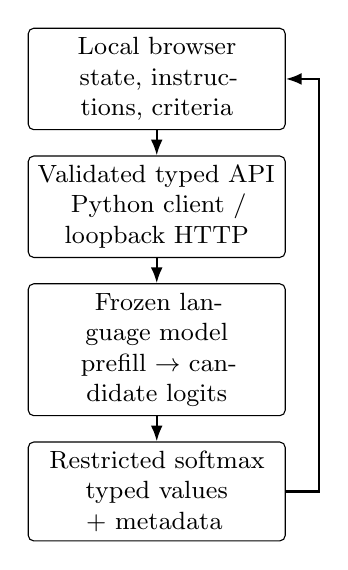
\begin{tikzpicture}[
  box/.style={draw,rounded corners=2pt,align=center,text width=3.03cm,minimum height=.72cm,font=\small},
  arr/.style={-{Latex[length=2mm]},thick},node distance=.32cm]
\node[box] (ui) {Local browser\\state, instructions, criteria};
\node[box,below=of ui] (api) {Validated typed API\\Python client / loopback HTTP};
\node[box,below=of api] (lm) {Frozen language model\\prefill $\rightarrow$ candidate logits};
\node[box,below=of lm] (readout) {Restricted softmax\\typed values + metadata};
\draw[arr] (ui)--(api);
\draw[arr] (api)--(lm);
\draw[arr] (lm)--(readout);
\draw[arr] (readout.east)--++(.42,0)|-(ui.east);
\end{tikzpicture}
\caption{The live demonstration uses the released typed API. It displays model-derived candidate distributions and typed values; no generated explanation or simulated prediction is inserted.}
\label{fig:architecture}
\end{figure}

\subsection{Relationship to one-token decoding}
Restricted softmax readout has the same mathematical candidate distribution as a sampler that masks all non-candidates, provided the model prefix, logits, candidate IDs, temperature, and other processors match. Greedy labels then agree unless tie-breaking differs; stochastic sampling agrees in distribution, not necessarily in realized samples. This is an equivalence under specified conditions, not a new inference theorem or learning method.

In particular, selecting a first token after prefill need not require another model forward pass. Avoiding a generated token therefore does not itself establish a speedup. The matched study in Section~\ref{sec:evidence} tests this point using an actual native one-token sampler, rather than comparing direct readout only with a long textual answer.

\section{Demonstration and Access}
\label{sec:demo}
The browser runs locally and connects through a small Python bridge to the existing model API. It requires no cloud inference service. A user starts with a shared state and three editable questions: routing through Choice, urgency through Noul, and priority through Score. The question instructions and criteria are visible, making the decision contract available for inspection before inference.

An example demonstration proceeds in four steps. First, the user reviews the state and defines what the available routes or stages mean. Second, \emph{Run decisions} submits the three questions and displays their typed values. Third, the user examines the candidate probabilities and compares a hard label with the distribution behind it; for Score, the expected stage and the most likely stage can differ. Finally, the user edits the state or a criterion and runs again, inspecting the new response. This is a way to explore behavior, not a controlled accuracy experiment: altering the prompt also alters the model input.

The page displays entropy concentration, measured elapsed time, and copyable request/response JSON. These serve different purposes. The bars explain which candidates receive relative model mass; the JSON exposes the software contract; elapsed time describes the current live request. None is a reference answer or an external quality score. The interface has no replay mode that could be mistaken for live inference. If the model API is unavailable, it reports an unavailable service instead of substituting a canned result.

% Root will add a verified live UI capture. Until then, the draft remains
% compilable without implying that a synthetic mockup is a real screenshot.
\IfFileExists{figures/demo-overview.png}{%
\begin{figure*}[t]
\centering
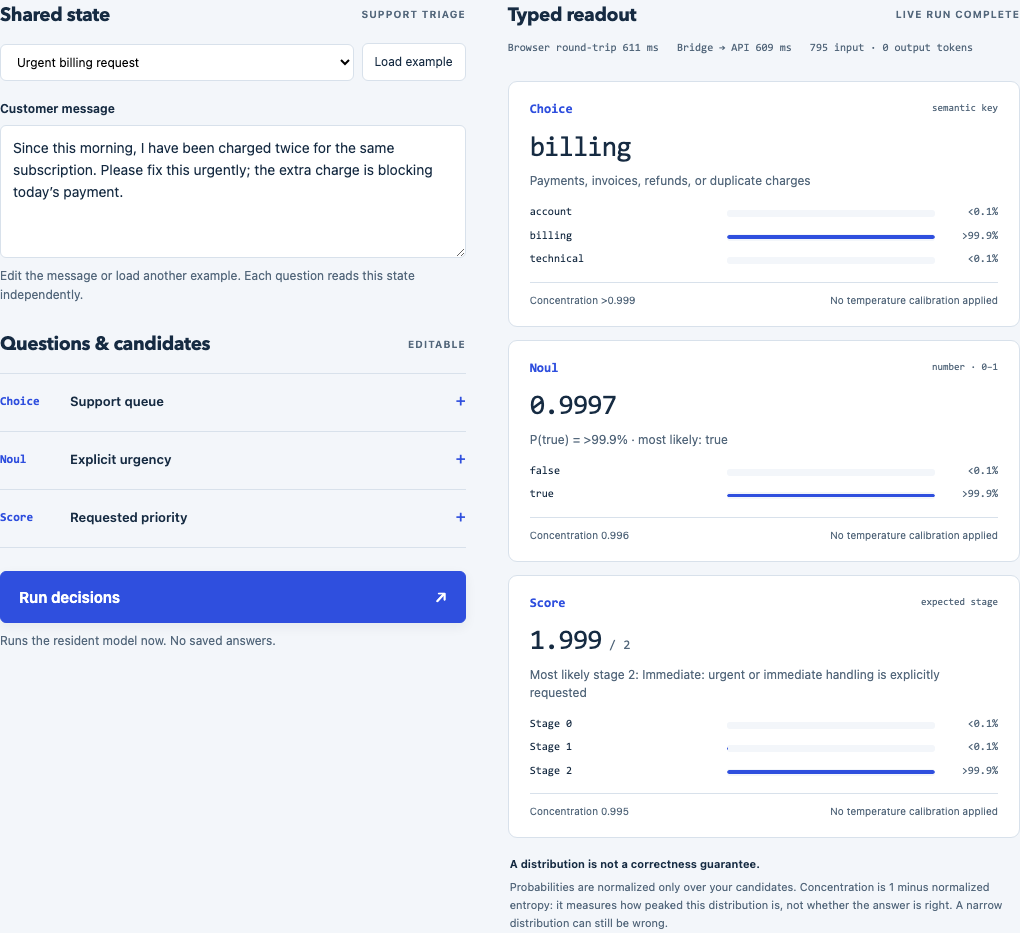
\includegraphics[width=\textwidth]{figures/demo-overview.png}
\caption{Live browser demonstration: editable inputs, typed outputs, and candidate distributions. The example illustrates the interface and is not an evaluation item.}
\label{fig:demo}
\end{figure*}}{}

Installation begins with the repository's native build script and pinned model downloader. Users build the helper with \texttt{build\_native.sh}, download the model with \texttt{fetch\_native\_model.py}, and start the API with \texttt{./run.sh --without-calibration}. Starting \texttt{python3 -m demo.server --port 8766} then opens access at \url{http://127.0.0.1:8766/}. The repository supplies complete commands and a Python client example. Fresh builds start at $T=1$; historical calibration artifacts are bound to their recorded runtime and should not silently transfer to a different build.

The tested environment is an Apple M5 Pro with 64\,GB unified memory and macOS 26.4, using Metal and Accelerate. The model file is approximately 20.4\,GB, in addition to runtime memory. This is a local workstation demonstration, not a claim of lightweight deployment or a demonstrated minimum-memory requirement. Source is distributed; model weights and compiled native binaries are not bundled.

\section{Evidence Behind the Demonstration}
\label{sec:evidence}
\subsection{Four distinct evidence sets}
Table~\ref{tab:sets} separates the evidence sources. Repeated runtime requests are not additional quality examples, and the external tasks do not share a single meaningful accuracy metric.

\begin{table}[t]
\centering
\small
\setlength{\tabcolsep}{3pt}
\begin{tabular}{@{}p{1.72cm}p{1.44cm}p{4.08cm}@{}}
\toprule
Evidence & Size & Interpretation \\
\midrule
Local regression & 2,400 items & Self-authored Japanese; 800 per type \\
Earlier JNLI & 300 items & Balanced public-development pilot \\
Expanded external & 600 items & JCoLA, JSTS, JCQA; 200 each \\
Matched runtime & 4,050 requests & 150 local $\times$ 5 repetitions, plus 600 external; 3 modes \\
\bottomrule
\end{tabular}
\caption{Distinct evidence sets. The matched study reuses the expanded external items and a subset of the local suite; these counts must not be added as independent evaluations. JCQA abbreviates JCommonsenseQA.}
\label{tab:sets}
\end{table}

The historical local suite contains 2,220 programmatically generated items from 45 template families and 180 individually AI-authored items. Its legacy \texttt{manual} field does not denote human annotation. AI agents reviewed the data, but there was no independent human annotation study. Authoring had access to some earlier development errors and retained related skill families; this suite is useful regression material, not a family-disjoint or fully blind external test.

The historical configuration returned valid typed responses for all 2,400 items and matched the designated top label on 2,238 (93.25\%). Type-specific results were 96.00\% Choice, 95.25\% Noul, and 88.50\% Score top-stage accuracy. The 162 errors despite valid outputs illustrate why the demo separates structure from correctness. Positive-temperature scaling fitted on a separate 120-item self-authored calibration split slightly improved aggregate NLL and Brier point estimates, but worsened ECE and Score expected-stage MAE. Concentration is consequently not presented as a generally validated correctness probability.

The earlier JNLI pilot selected 100 examples per class from public development data \citep{kurihara2022jglue}, obtaining 243/300 correct (81.0\%). Contradiction recall was only 61\%. Seventy-seven selected rows share an exact sentence with another selected row, so the pilot is not 300 independent linguistic contexts. It tests Choice on one task, not all three API types.

The expanded sample contains 200 examples each from JCoLA \citep{someya2024jcola}, JSTS, and JCommonsenseQA \citep{kurihara2022jglue}. Outcome-independent hash selection and task rubrics were frozen locally before inference; this was not independent preregistration. Public development data may have appeared in model training. Six JSTS rows share text or image provenance with the earlier JNLI selection, including three identical ordered sentence pairs. We record the overlap rather than claim four independent datasets.

\subsection{Matched runtime and parity}
All three conditions used one resident model and a common research HTTP response containing a type and semantic label. Direct readout and native one-token greedy selection used identical complete prompts and candidates. The JSON condition actually generated a grammar-constrained object, with a serialization-specific prompt. Its timing comparison therefore includes prompt and prefill differences as well as multi-token generation; it does not isolate sampler overhead.

The schedule contained $(150\times5+600)\times3=4{,}050$ measured requests, plus 21 synthetic warm-ups. All measured requests completed with valid responses and no recorded HTTP failures. Mode order was randomized within each item/repetition before execution. Timing ran from client serialization through loopback HTTP response parsing, with a persistent connection and Nagle's algorithm disabled. Native audit transfer and parsing were inside this interval; the subsequent trace-file write was outside it. These measurements describe the research harness, not the browser's full rendering time or a production service-level guarantee.

Direct and one-token conditions matched prompts, token sequences, candidate IDs, logits, and labels in all 1,350 paired observations. Maximum observed candidate-logit difference was zero; there were no maximum-logit ties. The primary latency statistic is the median across 150 local items of the within-item difference between five-repetition mean latencies. It is not a difference between marginal medians.

\begin{table}[t]
\centering
\small
\setlength{\tabcolsep}{3pt}
\begin{tabular}{@{}lrr@{}}
\toprule
Comparator $-$ direct & Difference & 95\% interval \\
\midrule
One token & $+0.0898$ & $[-0.7483,\;0.8449]$ \\
JSON & $+160.2958$ & $[138.1189,\;177.0587]$ \\
\bottomrule
\end{tabular}
\caption{Primary paired HTTP latency differences in milliseconds. Intervals resample observed local family/tag clusters; JSON uses a different serialization prompt.}
\label{tab:latency}
\end{table}

Table~\ref{tab:latency} gives 10,000-replicate whole-family/tag percentile intervals. They describe sensitivity to the observed cluster composition, conditional on this model, machine, selected items, and session. They do not estimate between-machine or independent-session variability. The one-token interval crosses zero: this run provides no evidence of a material direct-readout latency advantage. JSON was slower under its different serialization requirements, with task-dependent quality changes.

\subsection{External task-specific results}
Direct readout and one-token selection have identical external labels. JCoLA reached 86.0\% accuracy and MCC 0.5708; JSON reached 82.0\% and MCC 0.5160. The selected sample contains 158 acceptable sentences, so an always-acceptable rule already achieves 79.0\% accuracy and has undefined MCC. Reporting only accuracy would obscure this imbalance.

JCommonsenseQA accuracy was 95.0\% for direct/one-token and 95.5\% for JSON, a difference of one example. JSTS retains its continuous reference scores in $[0,5]$: direct expected-stage MAE at $T=1$ was 0.5065. JSON has no comparable probability vector, so we do not assign it an expected-stage metric. The separate hard-stage comparison gives MAE 0.5480 for direct/one-token and 0.5650 for JSON. We do not round the gold scores into invented classes or pool these tasks into one accuracy.

The release includes frozen protocols, selections, schedules, source/build hashes, request traces, task-specific analysis, and an independent AI-agent numerical audit. CPU analysis reconstructs published statistics without model execution. Reproduction of inference additionally requires upstream datasets, the pinned model, and a compatible runtime. A fresh build has its own artifact manifest; numerical and timing replication is not guaranteed across hardware or builds.

\section{Related Work and Scope}
Verbalizer-based classification predates this system \citep{schick2021pet}. Qwen3 rerankers provide a concrete precedent for next-token yes/no scoring \citep{zhang2025qwen3embedding,qwen3reranker}. Grammar-constrained decoding also produces structured outputs without task-specific finetuning \citep{geng2023grammar}; our JSON condition is a narrow comparator, not a comprehensive evaluation of constrained decoding.

Scalar temperature scaling \citep{guo2017calibration} changes distribution sharpness without changing the argmax. It is distinct from contextual calibration for prompt-induced label bias \citep{zhao2021calibrate}. Multiple-choice models can remain sensitive to option placement \citep{zheng2024selectors}. Canonical key ordering makes reversed dictionary insertion order equivalent in our software; it does not establish model invariance to semantically reordered options.

The demo's contribution is therefore inspectability and reproducible interface engineering. It neither introduces a new classifier nor establishes superiority over other typed-output systems. The released 35B configuration involves no decision-head training; a separate earlier small-model head experiment is documented in the repository and is not evidence of training gains for this system.

\section*{Limitations}
Evaluation uses one quantized model, one Apple Silicon device, and one matched execution session. Quality data are Japanese; an English interface example does not establish English task quality. The public external subsets are limited and have unknown training contamination. The local data were AI-authored and development-related, with no independent human reference validation. There is no user study establishing usability or downstream decision quality.

Candidate probabilities depend on prompts, labels, candidate coverage, and temperature. Concentrated wrong answers occur; neither type validity nor entropy concentration should trigger consequential actions without application-specific validation. Score assumes equally spaced stages and Noul is a relative candidate probability, not a verified frequency of truth. The model is large, questions run sequentially, and other operating systems or lower-memory configurations have not been validated. Live-demo elapsed time is not directly comparable with the research harness's controlled interval.

\section*{Ethics and Availability}
The demonstration is intended for inspecting model behavior and prototyping typed interfaces. It provides no evidence for high-stakes deployment. Live inference is local; users still remain responsible for the text they submit and any downstream use. The released code and self-authored local data use MIT terms. External-dataset-derived selection metadata, rubrics, protocols, and results retain the applicable CC BY-SA 4.0 attribution and share-alike terms, separately from generic code. Upstream dataset text, model weights, and compiled binaries are not bundled; the repository's data cards and notices specify acquisition and attribution.

\section*{Acknowledgements}
AI coding agents accessed through OpenAI Codex assisted with implementation, question authoring, software checks, experiment execution, analysis, literature organization, and manuscript drafting under the author's direction. The independent numerical audit was performed by another AI agent; it is not independent human review. We do not claim human-expert validation of the AI-authored evaluation items. The author is responsible for the submitted manuscript and its claims.

\bibliography{references}
\bibliographystyle{acl_natbib}
\end{document}
